\chapter{Background and Related Work}

In the following sections, we will present some background information and related work to our project. We will start by analyzing existing tools for debugging traditional web applications, including debugging tools that are integrated directly into browsers. We will also discuss some tools aimed at testing responsive web applications. Finally, we will present a few cross-device application development frameworks that either provide some cross-device testing mechanisms themselves or that could benefit from such mechanisms.

\section{Web Application Testing}

In the following subsections, we will present a few tools supporting the testing and debugging of traditional web applications. Those tools are clearly also relevant for cross-device applications, as most cross-device applications are web applications.

\subsection{Browser-Integrated Debugging Tools}

Over the last few years, browser manufacturers have added more and more tools for debugging web applications directly from the browser. Chrome arguably provides the most advanced debugging tools, but all browsers include at least basic tools for debugging web applications. We will now present a few of those tools provided by browsers themselves.

\subsubsection{Chrome DevTools}

Google Chrome provides a wide range of features for testing and debugging web applications. First of all, it lets the developer inspect the DOM tree of an application and allows on-the-fly editing of DOM elements. Furthermore, new CSS rules or properties can be added and existing ones can be modified. Figure~\ref{fig:chrome_devtools} shows a screenshot of the HTML and CSS inspector in Chrome DevTools. Another useful feature is the JavaScript Console. It has two main purposes: First, it can be used to log diagnostic information in the development process. Second, it is a shell prompt which can be used to interact with the document and DevTools. Chrome DevTools can also be used to debug JavaScript. It lists all scripts that are part of the inspected page. Breakpoints can be set in the scripts and standard controls to pause, resume and step through code are provided. All features mentioned before are also available for debugging remote devices. Remote debugging can be used by connecting a device to the desktop PC with a cable.

\begin{figure}[H]
  \centering
    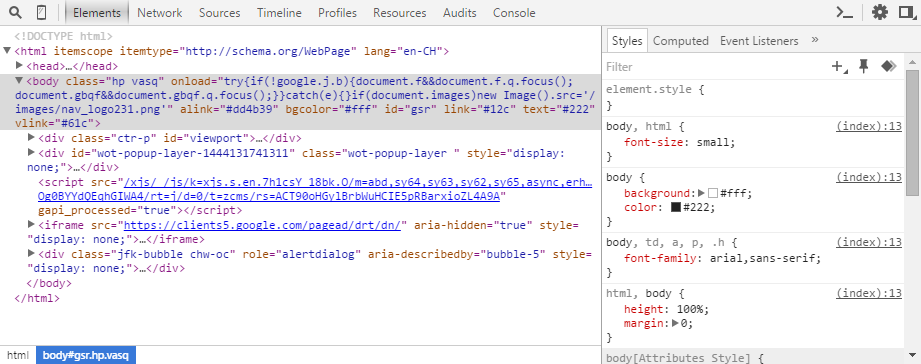
\includegraphics[width=1.0\textwidth]{images/relatedwork/chrome_devtools_3.png}
	\caption[Screenshot: Chrome DevTools]{HTML/CSS inspector of Chrome DevTools}
	\label{fig:chrome_devtools}
\end{figure}

Chrome DevTools provides many more features useful for debugging, but explaining them all would exceed the scope of this document. While all those features are very useful for testing and debugging web applications, their main disadvantage is that they can only be used to debug one device at a time.

\subsubsection{Firefox Developer Tools}

Firefox\footnote{\url{https://developer.mozilla.org/en-US/docs/Tools}} provides developer tools similar to Chrome DevTools. It also has a page inspector that allows developer to inspect the DOM tree and modify the CSS. It also features a console, a JavaScript debugger and remote debugging. Like Google Chrome's DevTools, Firefox's developer tools provides more features that we will not explain here. Furthermore, Firefox gives developers access to a feature called Developer Toolbar. The Developer Toolbar is a command-line tool that can be used to quickly access a number of Firefox's debugging tools. Overall, Chrome DevTools and Firefox Developer Tools are very similar and thus also have the same limitations. Just like Google Chrome, only one device can be debugged at a time in Firefox.

\subsubsection{Summary}

Internet Explorer\footnote{\url{https://msdn.microsoft.com/library/bg182326(v=vs.85)}}, Microsoft Edge\footnote{\url{https://msdn.microsoft.com/en-us/library/dn904498(v=vs.85).aspx}}, Opera\footnote{\url{http://www.opera.com/dragonfly/}}, Safari\footnote{\url{https://developer.apple.com/safari/tools/}} and other browsers all provide some kind of developer tools. However, they do not provide any features that we did not already mention before, thus we will not provide any detailed description of the developer tools available in those browsers. All those browsers share the same limitation: Their tools can only be used to debug one device at a time. For cross-device applications however, it would be desirable to debug multiple devices at a time without having to navigate between windows all the time.

\subsection{Record and Replay}

Record and replay has already successfully been used for debugging web applications. It allows developers to quickly reproduce bugs that are otherwise difficult to reproduce. Reproducing bugs in cross-device applications can be even more difficult than in traditional web applications because multiple devices and users are involved simultaneously. In the following, we will describe some tools that support record and replay in web applications.

\subsubsection{Timelapse}

In~\cite{timelapse2013}, Burg et al. describe their record and replay tool Timelapse. Timelapse is a tool for recording, reproducing, and debugging interactive behaviors in web applications. Timelapse is built on Dolos, a record/replay infrastructure that ensures deterministic execution by capturing and reusing user inputs, network responses, and other non-deterministic inputs. Developers can use Timelapse to browse, visualize, and seek within recorded program executions while simultaneously using familiar debugging tools such as breakpoints and logging. Figure~\ref{fig:timelapse} shows Timelapse. The developers of Timelapse conducted a user study with 14 web developers which showed no significant effect on task times, task success, or time spent reproducing behaviors when developers had access to Timelapse. Expert developers seemed to better integrate Timelapse into their workflow, using Timelapse to accelerate familiar tasks rather than redesigning their workflow. However, Timelapse distracted less-skilled developers that were led astray by unverified assumptions.

\begin{figure}[H]
  \centering
    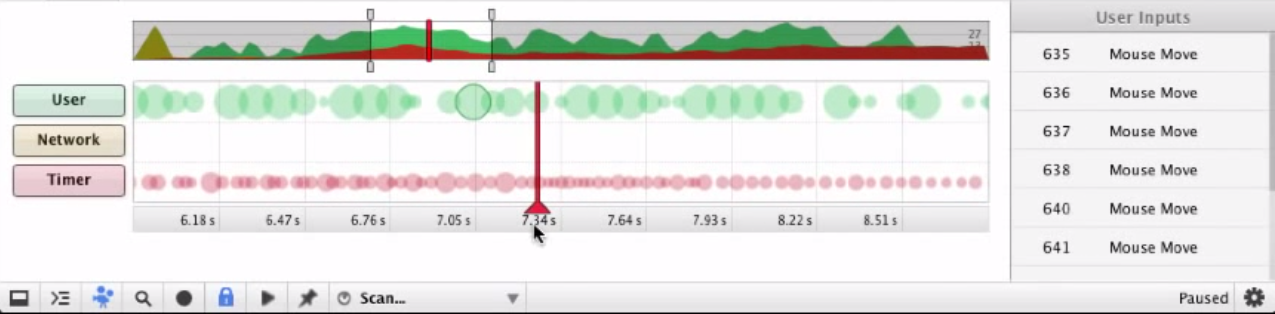
\includegraphics[width=1.0\textwidth]{images/relatedwork/timelapse.png}
	\caption[Screenshot: Timelapse]{Screenshot of Timelapse}
	\label{fig:timelapse}
\end{figure}

\subsubsection{Mugshot}

Mugshot, developed by Mickens et al.~\cite{mugshot2010}, is a record/replay system that captures all events in a JavaScript program, allowing developers to deterministically replay past executions of web applications. The goal of Mugshot is to provide low-overhead, "always-on" capture and replay for web-deployed JavaScript programs. Mugshot logs explicit user interactions like mouse clicks as well as background activities such as random number generation and the firing of timer callbacks. The client-side log is sent to the developer in response to a trigger like an unexpected exception being caught. The developer can then use Mugshot's replay mode to recreate the original JavaScript execution in his unmodified browser. 

\subsubsection{WaRR}

WaRR~\cite{warr2011} is a high-fidelity, "always-on" tool that records and replays the interactions between users and web applications. The WaRR recorder is embedded directly into the web browser and the WaRR Replayer uses an enhanced, developer-specific web browser that enables more realistic simulation of user interactions based on the recorded traces. Andrica et al. developed two tools on top of WaRR:
\begin{itemize}
	\item WebErr allows testing of web applications against human errors, i.e. navigation errors and timing errors.
	\item AUsER automatically generates user experience reports: If a user experiences a bug while using a web application, they press a button and the developers of the application receive the sequence of actions that led to the bug.
\end{itemize}
Using WebErr, the developers of WaRR were able to find a bug in Google Sites\footnote{\url{https://www.google.com/work/apps/business/products/sites/}}.

\subsubsection{Rumadai}

Yildiz et al.~\cite{rumadai2012} developed Rumadai, a Visual Studio plug-in that helps developers test web applications by recording and replaying client-side events. Rumadai injects JavaScript code into web pages to be deployed at servers. The injected code records user events as well as client-side dynamic content requests and their responses. The recorded events are sent to a database and can be queried by the developers of the web page. The recorded events can then be replayed in a browser using Rumadai seamlessly from Visual Studio.

\subsubsection{FireCrystal}

FireCrystal~\cite{firecrystal2009} is a Firefox extension that allows developers to extract the implementation details of interactive behaviors from other websites. Developers can tell FireCrystal to start recording and then demonstrate the interactive behavior they want to extract. FireCrystal records the interaction, keeping track of DOM changes, JavaScript executions and user input events. The developer can then replay the interactions and FireCrystal displays the HTML, CSS and JavaScript code that affected a particular element at any specific time. FireCrystal also provides an execution timeline that developers can scrub back and forth.

\subsubsection{Summary}

The tools described above all employ record and replay in some way for improving web applications. FireCrystal focuses more on extracting interactive behaviors from other websites, but it does so by providing record and replay mechanisms. The other tools all focus on debugging web applications. WaRR and Mugshot provide recording mechanisms directly to users of web applications, providing them with means of submitting bug reports to the developers of the applications. Some of those tools are designed for only replaying event sequences on the devices they were recorded on, while others allow replaying event sequences on different devices, e.g. the sequences can be replayed on the developer's machine after a user has recorded and submitted the bug. However, all of those tools have one limitation in common: They focus on replaying an event sequence on one device at a time. In cross-device scenarios, multiple devices can interact with the same application simultaneously and it would be desirable to replay interaction sequences on multiple devices in parallel.

Since record and replay mechanisms have already been shown to help with debugging in traditional web applications, they could certainly also be useful for debugging cross-device applications. In particular, we think that replaying event sequences on multiple devices simultaneously can help accurately simulate multiple users using a cross-device application. Developers usually work alone when fixing a bug, or in very small groups, which makes reproducing bugs that require multiple devices to interact with each other a very difficult task. However, if multiple devices replay event sequences simultaneously, mechanisms for accurately timing event execution are also required. Most of the tools described above do not include such mechanisms, or they include some mechanisms that are however not sufficient for configuring timing in a cross-device replaying scenario.

\section{Responsive Web Application Testing}

There are a number of tools for testing responsive websites. Some of them can be accessed on the web as a service, while others are desktop programs that have to be installed. Some focus on testing on real devices and others focus on emulating devices. In the following subsections we will describe some of those tools. Responsive web applications have a few similarities with cross-device applications: Both types of applications are supposed to work on a number of different devices with different screen sizes, input capabilities and more. Thus, tools for testing responsive web applications are to some extent also suited for testing cross-device applications.

\subsection{Web Services}

The following two tools can be accessed through a browser and do not have to be installed.

\subsubsection{BrowserStack}

BrowserStack\footnote{\url{https://www.browserstack.com/}} allows developers to select browsers and devices and then generate screenshots. It is also possible to live test one device at a time. Furthermore, there are developer tools for remote devices and Selenium cloud testing is possible. Even though BrowserStack allows the developer to see what an application looks like on many devices simultaneously, its usefulness for cross-device application testing is limited: Only one device can be live-tested at a time, making it difficult to accurately simulate a cross-device scenario. Also, even though real iOS devices are used, only emulated Android devices are available. One of the advantages of tools such as BrowserStack is that applications can be tested on many different real devices without having to buy those devices. Providing only emulated Android devices diminishes the usefulness of such a tool.

\subsubsection{CrossBrowserTesting}

With CrossBrowserTesting, developers can select a number of devices as well as the operating system, browser and resolution and generate screenshots. The layout differences between different devices can then automatically be analyzed. Furthermore, websites can also be live tested and Selenium automated testing is available as well. The main advantage of CrossBrowserTesting is that all screenshots are generated on real devices and a very wide variety of devices is available. Also, interactions can be tested using Selenium. The usefulness of the tool is again limited by the fact that live testing is only possible on one device at once. Additionally, while detecting layout differences is a useful feature in general, it is not yet very mature and some layout differences that are detected seem rather trivial (the body element of a larger device is larger), while other differences are not noticed at all. Figure~\ref{fig:crossbrowsertesting} shows CrossBrowserTesting while taking screenshots on multiple devices.

\begin{figure}[H]
  \centering
    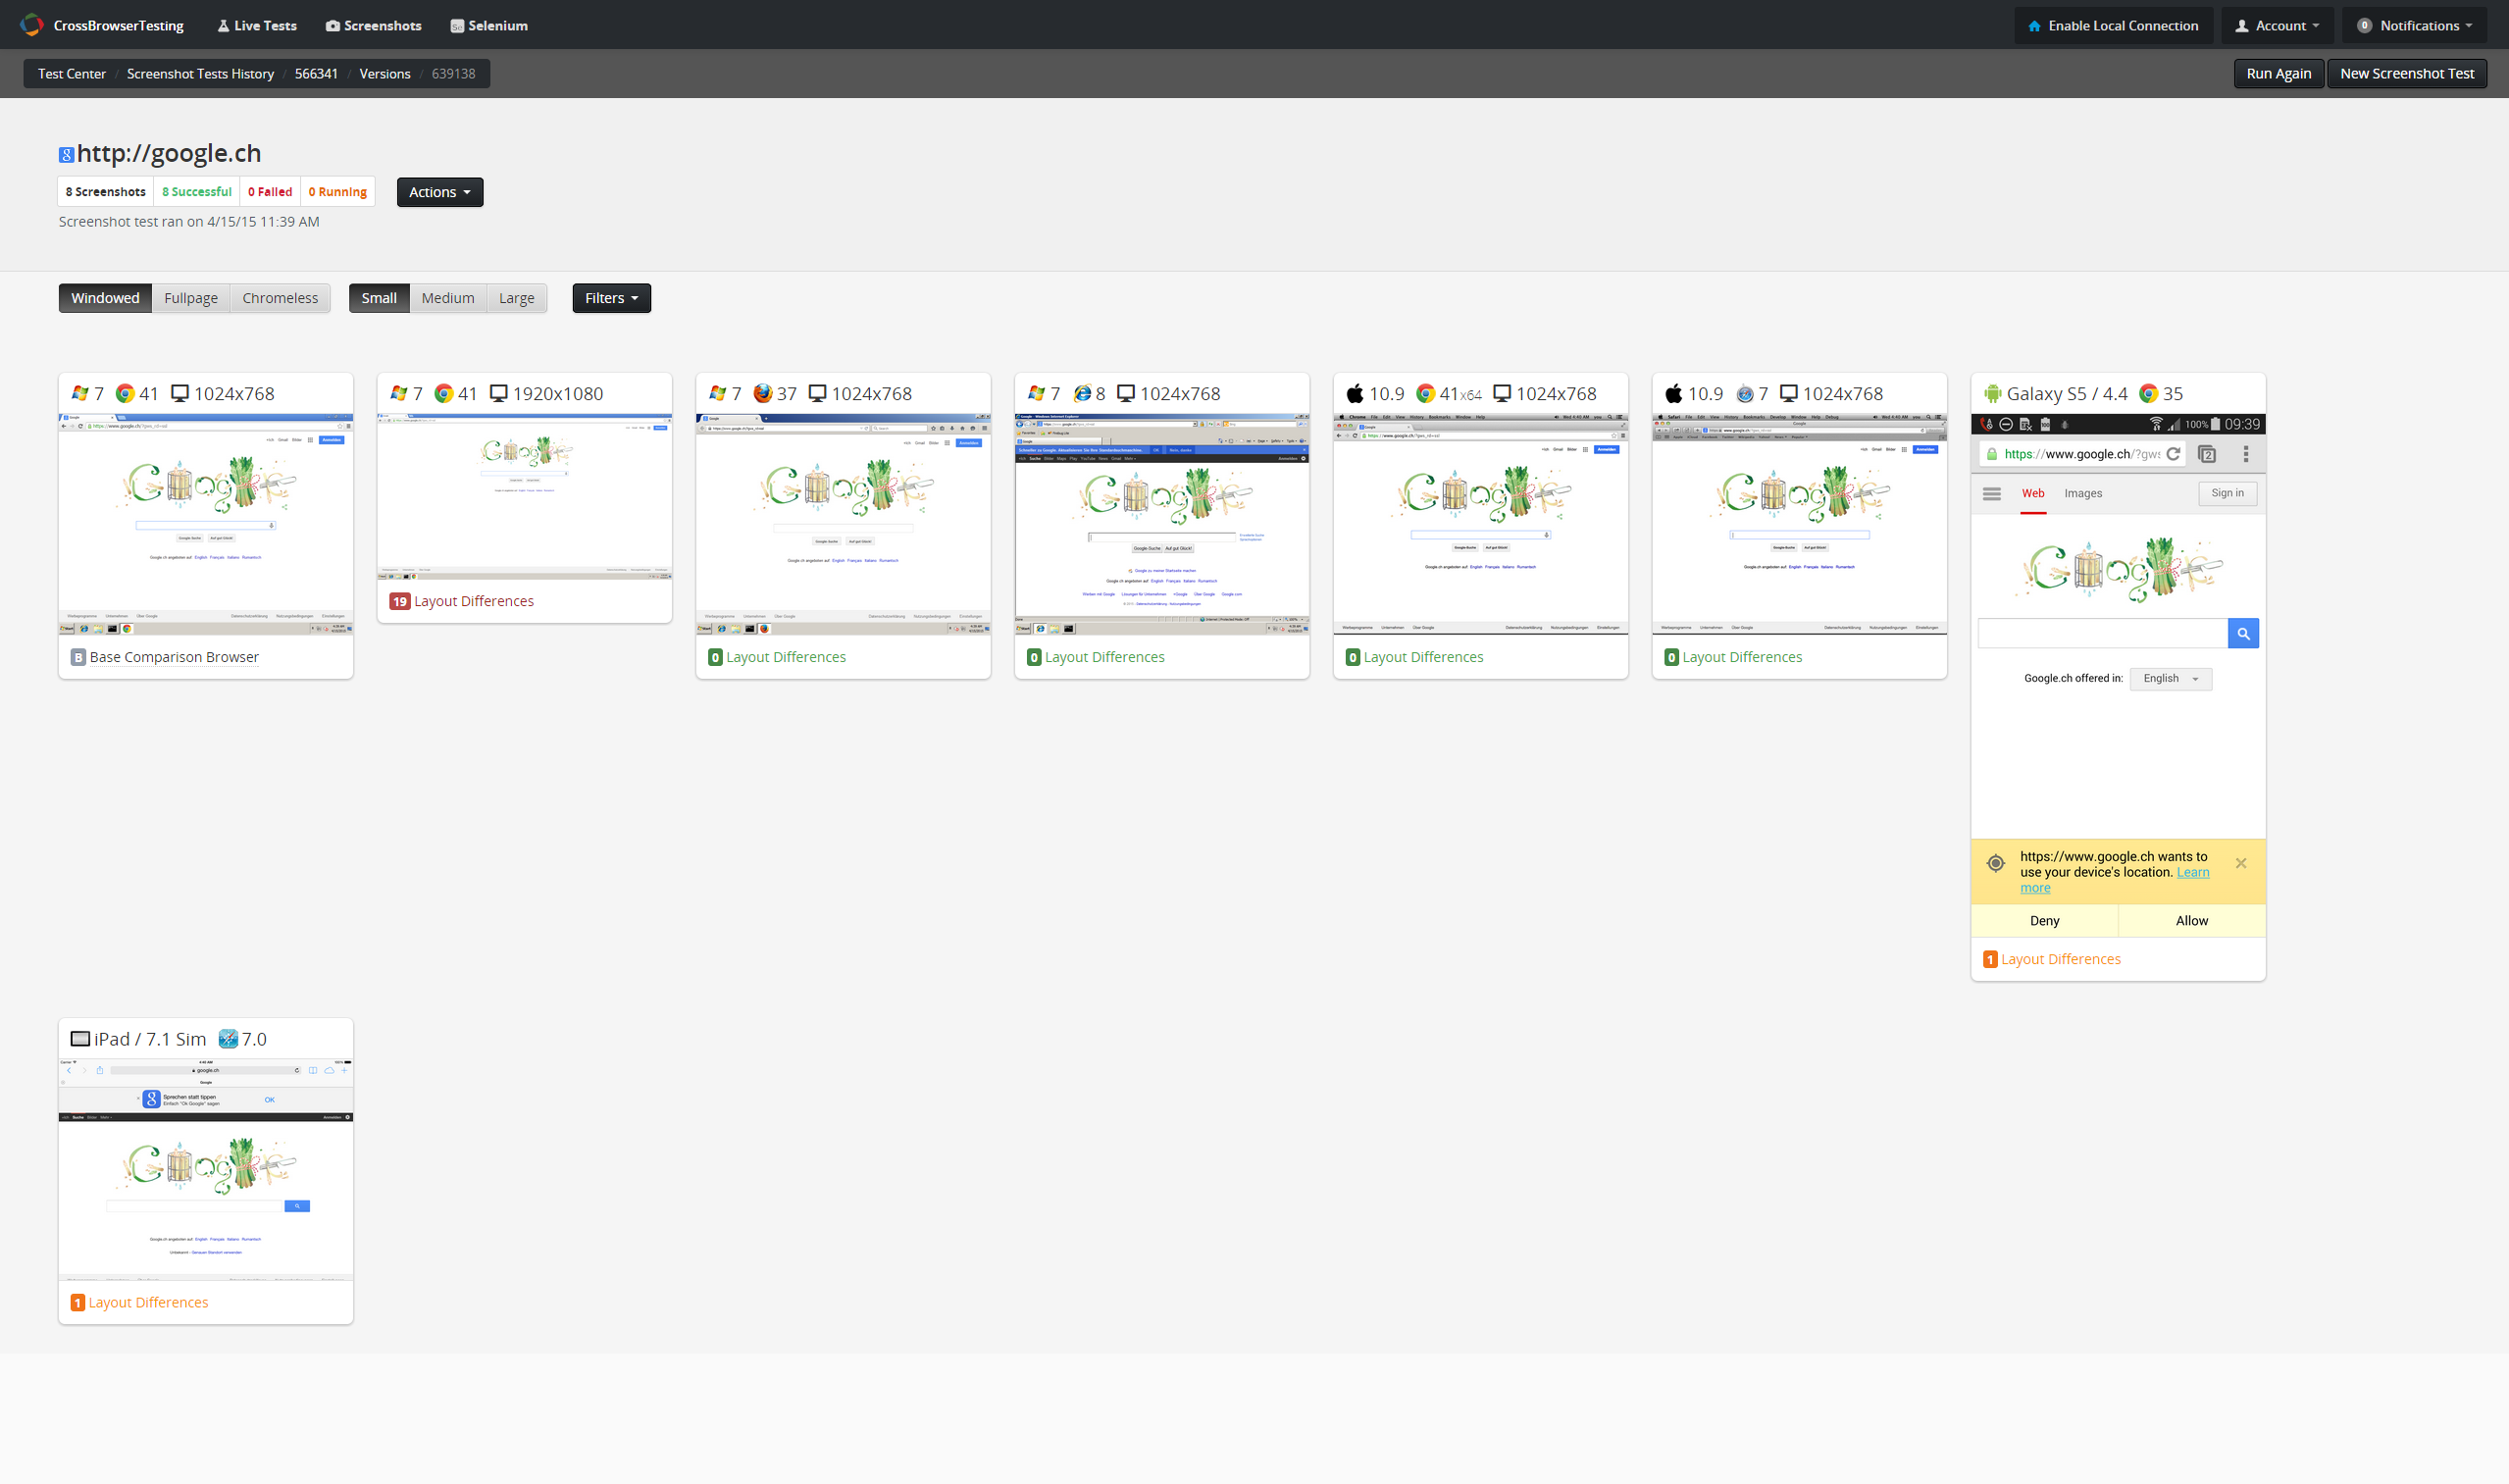
\includegraphics[width=1.0\textwidth]{images/relatedwork/cross_browser_testing.png}
	\caption[Screenshot: CrossBrowserTesting]{Taking screenshots on multiple devices simultaneously}
	\label{fig:crossbrowsertesting}
\end{figure}

\subsection{Testing with Actual Devices}

The following tools allow the developer to connect multiple real devices to the tool and test their application on them.

\subsubsection{Remote Preview}

Remote Preview\footnote{\url{https://github.com/viljamis/Remote-Preview}} allows synchronizing URLs across multiple devices. This allows fast previewing of a web application on multiple devices. In cross-device scenarios, loading the same URL on all devices can help in applications where devices are paired by opening the same URL on all devices. However, Remote Preview provides a rather limited set of features, thus using Remote Preview alone will probably rarely be enough for successfully testing web applications.

\subsubsection{BrowserSync}

BrowserSync (see Figure~\ref{fig:browsersync}) provides a large number of features for testing websites. It allows remote debugging of HTML and CSS, can add CSS outlines or box shadows to all elements and add a CSS grid overlay. It can also load a URL on all devices, refresh all devices and automatically refresh devices when files are changed. Furthermore, it allows synchronizing interactions between devices, i.e. clicks, scrolls, form submits, form inputs and form toggles. It also provides network throttling. The advantages of BrowserSync are that it provides a wide range of features, including synchronizing interactions, which is a feature that distinguishes it from many other tools. However, for cross-device application testing, synchronizing interactions among all devices is of limited usefulness, as different devices have different roles and thus also different responsibilities.

\begin{figure}[H]
  \centering
    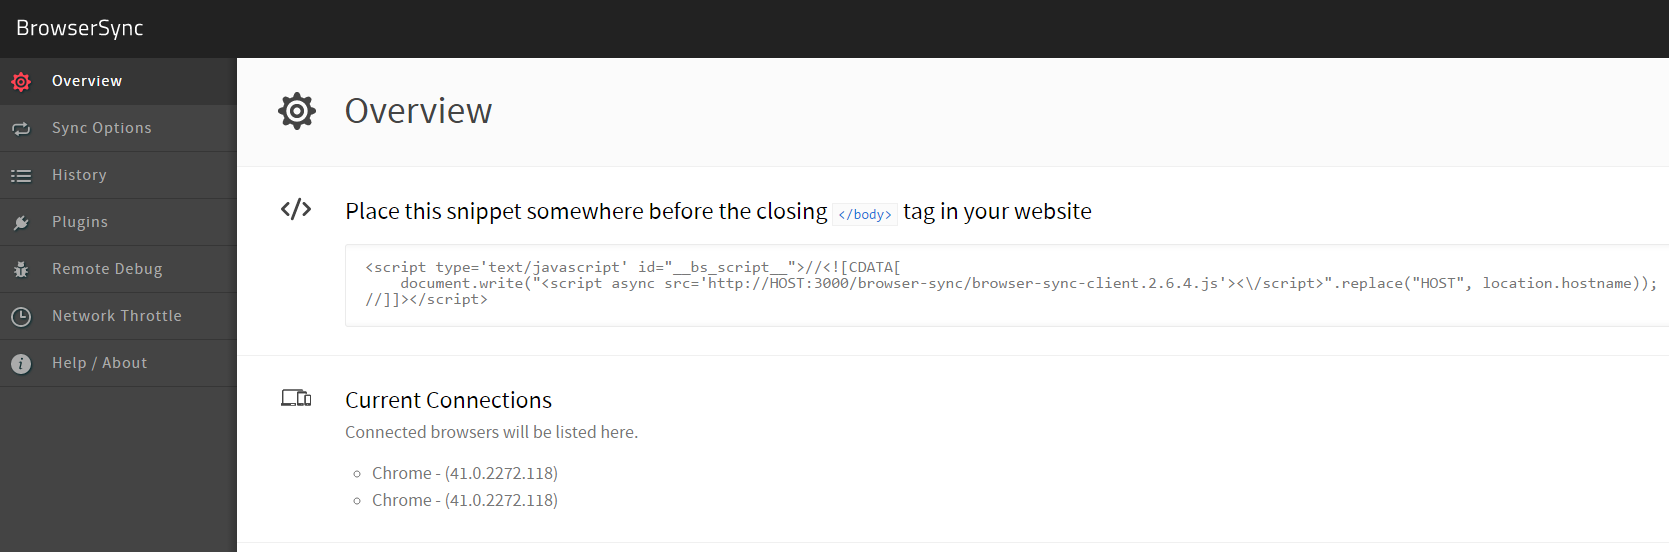
\includegraphics[width=1.0\textwidth]{images/relatedwork/browser_sync_3.png}
	\caption[Screenshot: BrowserSync]{Screenshot of BrowserSync}
	\label{fig:browsersync}
\end{figure}

\subsubsection{Adobe Edge Inspect CC}

Adobe Edge Inspect CC allows developers to take screenshots on all connected devices simultaneously. The screenshots are then automatically transferred to a folder on the desktop PC. It can also refresh all devices simultaneously. Furthermore, the URL that is opened on the desktop PC is loaded on all other connected devices. It also allows remote HTML and CSS debugging using weinre\footnote{\url{https://people.apache.org/~pmuellr/weinre-docs/latest/}}. The main advantage that distinguishes Adobe Edge Inspect CC from other tools is that is simply synchronizes the URL that the developer is currently looking at on the desktop PC, thus it works even if the developer switches tabs or browser windows. However, the fact that the URL cannot be changed from devices other than the desktop PC could be a disadvantage in some scenarios. Also, the installation process is rather extensive: A program needs to be installed on the desktop PC as well as a Chrome extension and an app needs to be installed on all mobile devices that the developer wants to connect. Regarding cross-device applications, again, refreshing all devices at once can be useful as well as synchronizing URLs in some cases, but other than that, it does not provide any features that help with cross-device application testing.

\subsubsection{Ghostlab}

Ghostlab\footnote{\url{http://www.vanamco.com/ghostlab/}} is one of the most advanced tools for responsive web application testing and provides features similar to BrowserSync. It can also load a URL on all devices or refresh all devices at once and refresh automatically when files are changed. It provides means for synchronized browsing as well as synchronized HTML and CSS inspection on multiple devices. Furthermore, it can automatically fill out forms and provides remote Javascript debugging. Synchronization can be turned on and off on a per-device basis, which makes the tool more useful than tools that simply synchronize all devices. However, the usefulness is still limited because constantly changing the devices that should be synchronized is time-consuming and error-prone. Also, interactions on cross-device applications typically do not happen in a synchronous fashion.

\subsection{Device Emulation}

The following tools allow the developer to emulate mobile devices on a desktop PC. 

\subsubsection{Chrome Device Mode}

Google Chrome provides extensive support for emulating devices with its Device Mode (see Figure~\ref{fig:device_mode}). If the developer opens the DevTools, they can switch to the Device Mode and emulate different devices. The developer can select an arbitrary device from a list of predefined devices or create a custom device. They can also enable network throttling, touch emulation and location emulation. The large number of different aspects that are emulated in Device Mode make it very well suited  for testing responsive web applications. While most other device emulation tools are limited to emulating resolution and sometimes touch, Chrome Device Mode allows to emulate many other aspects as well.

\begin{figure}[H]
  \centering
    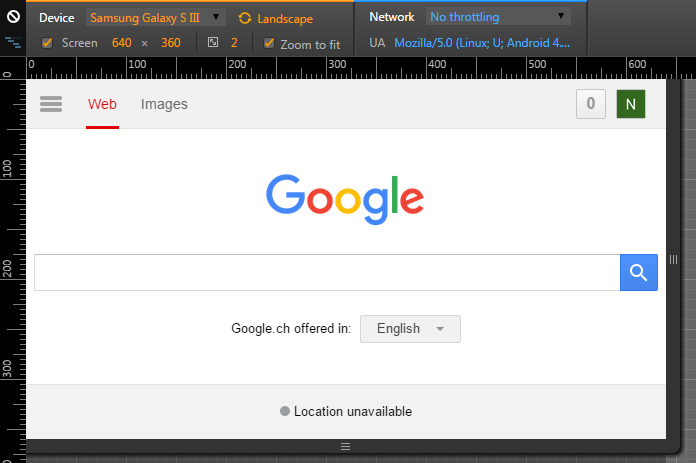
\includegraphics[width=0.8\textwidth]{images/relatedwork/device_mode_2.png}
	\caption[Screenshot: Chrome Device Mode]{Screenshot of Chrome Device Mode}
	\label{fig:device_mode}
\end{figure}

\subsubsection{Firefox's Responsive Design View}

Firefox's Responsive Design View also allows developers to emulate devices, similar to Chrome's Device Mode, but it provides fewer features. Instead of focusing on existing devices, it provides a short list of common resolutions that can be selected by the developer. It also allows to emulate a custom resolution. Additionally, the orientation of the devices can be switched, touch can be emulated, and screenshots of the displayed web page can be taken.

\subsection{Summary}

While the tools described above already provide a wide variety of features that are immensely useful for responsive web application testing as well as web application testing in general, the distinguishing characteristics of cross-device applications lead to a limited usefulness of those tools. In summary, there are two different approaches to testing cross-device applications in the tools described above: First, applications can be tested on real devices, either through web services or the developer's own real devices. Second, emulated devices can be used. In most of those tools, only one device can be tested at a time, but in cross-device scenarios, multiple devices are typically involved. In some of the tools, interactions can be synchronized among multiple connected real devices. However, this is also problematic for testing cross-device applications because not all devices perform the same interactions and those that do, do not necessarily perform them at exactly the same time. Two features that some of the tools mentioned above provide and that would definitely also be useful for cross-device applications are refreshing all devices at once and loading a URL on all devices. Remote HTML, CSS and JavaScript debugging are also desirable in a cross-device scenario. Something similar to Selenium testing is clearly also useful in cross-device scenarios. However, depending on the device, different tests would be needed and it should be possible to run those tests in parallel.

\section{Cross-Device Application Development Frameworks}

In the following subsections, we will describe some frameworks that facilitate the development of cross-device applications. Some of those frameworks already provide some basic mechanisms for testing the applications developed with them, but others include none and could benefit a lot from such mechanisms.

\subsection{Frameworks that have some Testing Tools}

The following frameworks already include some mechanisms for testing and debugging applications, but most of those mechanisms are limited to specific aspects of the applications and require the applications to be developed with the framework.

\subsubsection{XDStudio}

In ~\cite{xdstudio2014}, Nebeling et al. present their web-based GUI builder, XDStudio (see Figure~\ref{fig:xdstudio}). XDStudio is designed to support interactive development of cross-device web interfaces. It has two complementary authoring modes: \emph{Simulated authoring} allows designing for a multi-device environment on a single device by simulating other target devices. \emph{On-device authoring} allows the design process itself to be distributed over multiple devices. The design process is still coordinated by a main device, but directly involves target devices. The user can switch between two different modes: In \emph{use mode}, the user can interact normally with the interface loaded into the editor. In \emph{design mode}, the user can manipulate the interface directly. XDStudio also allows the specification of \emph{distribution profiles} in terms of involved devices, users and target user interfaces.

\begin{figure}[H]
  \centering
    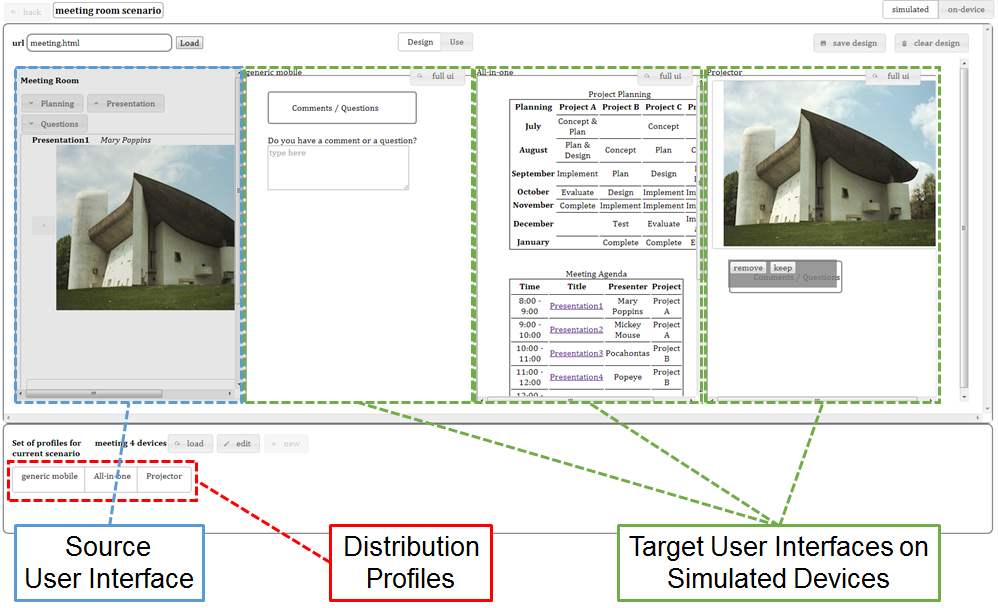
\includegraphics[width=0.8\textwidth]{images/relatedwork/xdstudio.png}
	\caption[Screenshot: XDStudio]{Screenshot of XDStudio}
	\label{fig:xdstudio}
\end{figure}

Although XDStudio includes mechanisms for inspecting interactive designs on emulated devices and on connected real devices, there is no specific support for debugging such as access to the console. Thus, XDStudio is well suited for seeing what an application looks and feels like on different devices, but debugging the application when something does not work as expected is still a difficult task.

\subsubsection{XDSession}

XDSession, developed by Nebeling et al.~\cite{xdsession2015}, is a framework for cross-device application development based on the concept of \emph{cross-device sessions}. The session controller supports management and testing of cross-device sessions with \emph{connected or simulated devices} at run time. The session inspector enables inspection and analysis of multi-device/multi-user sessions with support for \emph{deterministic record and replay} of cross-device sessions. A session consists of users, devices, and information.

XDSession provides a capture and replay mechanism for user interactions and changes to sessions and provides a basic device emulation mode that allows developers to emulate one device at a time. However, the record and replay mechanism only works if the framework's API is used for the manipulations. Also, XDSession supports debugging at a rather high level of abstraction and is thus better suited for finding problems in interactions rather than bugs in the source code.

\subsubsection{Weave}

Weave is a web-based framework for creating cross-device \emph{wearable} interaction by scripting, developed by Chi et al.~\cite{weave2015}. It provides a set of high-level APIs for developers to easily \emph{distribute UI output} and \emph{combine sensing events and user input} across mobile and wearable devices. Devices can be manipulated regarding their capabilities and affordances, rather than low-level specifications. Weave also has an integrated authoring environment for developers to program and test cross-device behaviors. Developers can test their scripts based on a set of simulated or real wearable devices.

Weave allows testing on emulated and real devices and the developer also has access to a log panel, but no further support for debugging is provided. 

\subsubsection{WatchConnect}

In ~\cite{watchconnect2015}, Houben et al. present WatchConnect. WatchConnect is a toolkit for rapidly prototyping cross-device applications and interaction techniques with smartwatches. It provides an \emph{extendable hardware platform} that emulates a smartwatch, a \emph{UI framework} that integrates with an existing UI builder and a rich set of \emph{input and output events} using a range of built-in sensor mappings. WatchConnect is built around a wired prototyping watch, a smart watch emulator composed of a display, a number of sensors and a microprocessor. Applications can thus be tested and debugged directly on the watch prototype. WatchConnect also includes some tools for supporting developers while debugging, but those tools are focused on the machine learning algorithms and the recording of sensor data.

\subsection{Frameworks that would Benefit from Testing Tools}

The following frameworks allow developers to develop cross-device web applications but include no tools for testing and debugging the applications developed with them and would certainly benefit from such tools.

\subsubsection{XD-MVC}

XD-MVC is a framework that combines cross-device capabilities with MVC frameworks. It can be used as a plain JavaScript library or in combination with Polymer. The framework consists of a server-side and a client-side part. For communicating, either a \emph{peer-to-peer} or a \emph{client-server} approach can be used. Developers that use XD-MVC can assign \emph{roles} to devices that are connected to the application. Depending on the role that a device is assigned, different parts of the interface are shown on the device. 

\subsubsection{Connichiwa}

Connichiwa by Schreiner et al.~\cite{connichiwa2015} is a framework for developing cross-device web applications. It runs local web applications on one of the devices without requiring an existing network or internet connection. \emph{No remote server} is used, instead a native helper-application runs a web server on-demand. The native application automatically \emph{detects other devices} using Bluetooth Low Energy, which are then connected by sending the IP address of the local web server over Bluetooth. Connichiwa's \emph{JavaScript API} gives easy access to common functions like device detection and connection and it also provides JavaScript events to notify about device detection and connection.

\subsubsection{DireWolf}

DireWolf is a framework for developing distributed web applications based on widgets. It was developed by Kovachev et al.~\cite{direwolf2013}. Direwolf provides a \emph{framework for easy browser-based distribution} of web widgets between multiple devices, facilitates extended \emph{multi-modal real-time interactions} on a federation of personal computing devices and provides \emph{continuous state-preserving widget migration}. DireWolf helps managing a set of devices and handles communication and control of distributed parts of the web application. 

\subsubsection{Panelrama}

Panelrama, developed by Yang et al.~\cite{panelrama2014}, is a web-based framework for the construction of applications using distributed user interfaces. It introduces a new \emph{XML element}, "panel", which may be placed around groupings of control and it facilitates the \emph{distribution and synchronization of panels} among the connected devices. The developer can specify the \emph{state information} that should be synchronized across devices as well as the suitability of panels to different types of devices. An \emph{optimization algorithm} distributes panels to devices that maximize their match for the developer's intent.

\subsubsection{Polychrome}

Polychrome is a web application framework for creating web-based collaborative visualizations that can span multiple devices. It was developed by Badam et al.~\cite{polychrome2014}. It supports co-browsing new web applications as well as legacy websites with \emph{no migration costs}, an \emph{API to develop new web applications} that can synchronize the UI state on multiple devices to support synchronous and asynchronous collaboration and \emph{maintenance of state and input events} on a server to handle common issues with distributed applications. Polychrome provides the interaction and display space distribution mechanisms to create new collaborative web visualizations that utilize multiple devices and it provides framework modules to store the user interaction. Combined with the initial state of the website, the interaction logs are useful for synchronizing devices within the collaborative environment, consistency management and interaction replay.

\subsection{Summary}

In the sections above, we have described several different frameworks for developing cross-device applications. Some of them are only useful for specific types of applications, while others are suited for cross-device applications of all types. Despite this abundance of frameworks available, little support for testing and debugging the applications that are developed with them is provided. DireWolf, Polychrome and XD-MVC include no mechanisms for testing and run in an unmodified browser. Thus, they could benefit from a web-based tool for testing cross-device applications. Panelrama applications also run in an unmodified browser. The developers of Panelrama mention that a tool for simulating device configurations and previewing the distribution was built on request of some developers. No further details about the tool were mentioned, but the fact that developers requested such a tool shows that it is often difficult to imagine what an application would look like on different device configurations. Thus, the developers of Panelrama applications would certainly also benefit from a cross-device testing tool. Connichiwa requires the installation of a helper application, but the application itself still runs in an unmodified browser. Thus, applications developed with Connichiwa could also be tested with a web-based cross-device testing tool.

Some of the frameworks above allow the emulation of devices as well as the connection of real devices. Emulating multiple devices at a time as well as connecting real devices is a crucial feature for testing and debugging cross-device applications, but without any additional tools that help with debugging, finding and fixing bugs in the applications is still a difficult task. The framework that provides the most support for testing so far is probably XDSession, but as described above, its mechanisms are still not enough for successfully debugging cross-device applications at the source code level.